\documentclass[10pt,twocolumn]{article}

\usepackage[utf8]{inputenc}
\usepackage[T1]{fontenc}
\usepackage[margin=0.75in]{geometry}
\usepackage{amsmath,amssymb}
\usepackage{graphicx}
\usepackage{booktabs}
\usepackage{hyperref}
\usepackage{xcolor}
\usepackage{listings}
\usepackage{algorithm}
\usepackage{algpseudocode}
\usepackage{multirow}
\usepackage{abstract}
\usepackage{enumitem}
\usepackage{subcaption}

\hypersetup{colorlinks=true, linkcolor=blue, citecolor=blue, urlcolor=blue}

\lstset{
  language=Python,
  basicstyle=\ttfamily\scriptsize,
  keywordstyle=\color{blue}\bfseries,
  stringstyle=\color{red},
  commentstyle=\color{gray}\itshape,
  showstringspaces=false,
  frame=single,
  breaklines=true,
  numbers=left,
  numberstyle=\tiny\color{gray},
  xleftmargin=2em,
  framexleftmargin=1.5em,
}

\title{AutoLineage: Zero-Code In-Memory Data Lineage Tracking for Machine Learning Pipelines}

\author{}
\date{}

\begin{document}
\maketitle

% ============================================================
\begin{abstract}
Reproducibility remains a critical challenge in machine learning, with studies showing that a significant fraction of published results cannot be independently verified. A key factor is the absence of automated data lineage tracking: practitioners rarely document transformations applied during pipeline development, and existing tools require manual logging or code restructuring. We present \textbf{AutoLineage}, a Python library that automatically captures fine-grained, in-memory data lineage by hooking into pandas DataFrame operations at runtime. Unlike prior tools that track only file-level inputs and outputs, AutoLineage records each transformation along with its parameters, shape changes, and column-level modifications---without requiring any code changes.

We conduct a comprehensive evaluation: (1)~two real-world ML pipelines demonstrating lineage capture across regression and classification tasks; (2)~a comparative analysis showing AutoLineage captures 14/14 pipeline steps versus 2/14 for MLflow and 1/14 for DVC; (3)~a correctness validation achieving 100\% recall and 100\% shape accuracy; (4)~performance benchmarks showing median overhead of $\sim$1~ms per operation; and (5)~a preliminary user study with $n$ practitioners comparing debugging efficiency across tools. AutoLineage is open-source and available on PyPI.
\end{abstract}

\par\noindent\textbf{Keywords:} data lineage, reproducibility, machine learning, data provenance, MLOps

% ============================================================
\section{Introduction}
\label{sec:intro}

The reproducibility crisis in machine learning is well-documented and growing. Pineau et al.~\cite{pineau2021} found that a substantial portion of ML papers lack sufficient detail to reproduce results. Gundersen and Kjensmo~\cite{gundersen2018} reported that fewer than 25\% of surveyed AI papers met basic reproducibility criteria. Sculley et al.~\cite{sculley2015} identified data dependencies as the most insidious form of technical debt in ML systems---unlike code dependencies, data transformations are difficult to detect and costly to reconstruct.

The problem is not merely academic. Paleyes et al.~\cite{paleyes2022} surveyed ML deployment case studies and found data pipeline issues among the top challenges. Amershi et al.~\cite{amershi2019} reported that at Microsoft, data-related activities consume the largest fraction of ML engineering effort. Sambasivan et al.~\cite{sambasivan2021} coined the term ``data cascades''---compounding errors from poor data practices---and found they affect 92\% of organizations deploying AI. Organizations face regulatory pressure to document data processing chains: the EU AI Act (Articles~10 and~17) requires high-risk AI systems to maintain records of data governance~\cite{veale2021}, and documentation frameworks like Model Cards~\cite{mitchell2019} and Datasheets for Datasets~\cite{gebru2021} have become community standards.

\subsection{The Code--Lineage Gap}

At the core of this problem is a fundamental asymmetry: \emph{code tells you what could have happened; lineage tells you what actually happened in a specific run.} Consider a preprocessing script with conditional cleaning:

\begin{lstlisting}[numbers=none,caption={The same code produces different lineage depending on runtime data conditions.},label={lst:codegap}]
null_rate = df.isnull().mean().max()
if null_rate > 0.05:
    df = df.dropna()       # Path A: drop 500 rows
else:
    df = df.fillna(median)  # Path B: impute 100 vals

q99 = df['value'].quantile(0.99)
if q99 > 1000:
    df = df[df['value'] < q99]  # Conditional filter

if 'category' in df.columns:
    df = pd.get_dummies(df)     # One-hot encode
else:
    df = df.assign(cat_flag=0)  # Placeholder
\end{lstlisting}

Running this script on two datasets produces entirely different transformation chains: one run drops rows, filters outliers, and adds 5~columns; another imputes values, skips filtering, and adds 1~column. The output shapes differ by thousands of rows and multiple columns. Yet the code is identical, the DVC pipeline definition is unchanged, and MLflow logs the same experiment structure for both runs.

Only \emph{runtime lineage tracking} captures these distinctions.

\subsection{Existing Tool Limitations}

Current tools address fragments of the lineage problem:

\textbf{MLflow}~\cite{zaharia2018} provides experiment tracking with APIs for logging parameters, metrics, and artifacts. However, it requires explicit instrumentation (typically 10--20 lines of \texttt{log\_param}/\texttt{log\_metric} calls) and does not track in-memory DataFrame operations. A script that reads a CSV, applies five transformations, and writes the result appears as a single experiment run with user-selected metadata.

\textbf{DVC}~\cite{kuprieiev2021} versions data files and defines reproducible pipelines via YAML. It tracks file-level dependencies between pipeline stages but is blind to operations within a stage. DVC knows that \texttt{clean.py} depends on \texttt{data.csv} and produces \texttt{clean.csv}; it does not know what transformations occurred inside \texttt{clean.py}.

\textbf{Weights \& Biases}~\cite{wandb2020} provides enhanced experiment visualization but shares MLflow's fundamental limitation: manual instrumentation with no in-memory tracking.

None of these tools record what happens \emph{between} a file read and a file write---precisely where most data transformations occur.

\subsection{Contributions}

We present \textbf{AutoLineage} with four contributions:

\begin{enumerate}[leftmargin=*, nosep]
  \item \textbf{Zero-code tracking}: A single import (\texttt{import autolineage.auto}) installs hooks on 25+ pandas operations, requiring no decorators, config files, or API calls.
  
  \item \textbf{In-memory transformation tracking}: Captures each DataFrame operation with its parameters, input/output shapes, column-level diffs, and row-count changes---granularity not available in any existing ML tool.
  
  \item \textbf{Comprehensive evaluation}: Two real-world pipelines, a comparative analysis against MLflow and DVC, a ground-truth correctness validation (100\% recall, 100\% shape accuracy), performance benchmarks, and a preliminary user study.
  
  \item \textbf{Open-source tool}: Published on PyPI (v0.2.0), MIT-licensed, with 34 passing tests and CI/CD via GitHub Actions.
\end{enumerate}

% ============================================================
\section{Related Work}
\label{sec:related}

\subsection{ML Reproducibility}

The reproducibility crisis spans both academia and industry. Gundersen and Kjensmo~\cite{gundersen2018} surveyed 400 AI papers across top venues and found that most failed to report sufficient experimental details. Pineau et al.~\cite{pineau2021} proposed a reproducibility checklist subsequently adopted by NeurIPS and ICML. While these documentation standards improve reporting, they do not provide automated tooling---compliance remains a manual effort that degrades over time.

The problem extends beyond research. Polyzotis et al.~\cite{polyzotis2018} identified data lifecycle management as a first-class challenge in production ML, noting that ``data management is the most under-appreciated aspect of ML.'' Shankar et al.~\cite{shankar2022} interviewed ML engineers and found that most debugging time is spent tracing data issues. Renggli et al.~\cite{renggli2021} proposed a data quality-driven view of MLOps where automated provenance is essential for continuous monitoring.

\subsection{Experiment Tracking}

MLflow~\cite{zaharia2018} is the most widely adopted experiment tracking framework. Its tracking API provides four abstractions: runs, parameters, metrics, and artifacts. A typical instrumented script requires 10--20 additional lines of code:

\begin{lstlisting}[numbers=none]
import mlflow
mlflow.start_run()
mlflow.log_param("n_estimators", 200)
mlflow.log_param("test_size", 0.2)
# ... pipeline code ...
mlflow.log_metric("rmse", rmse)
mlflow.log_artifact("model.pkl")
mlflow.end_run()
\end{lstlisting}

This captures experiment-level metadata but nothing about data transformations. If \texttt{dropna} removes 207~rows, this fact is lost unless the user manually adds \texttt{mlflow.log\_metric("rows\_after\_dropna", len(df))}.

Weights \& Biases~\cite{wandb2020} provides similar functionality with enhanced visualization. Both tools operate at the experiment level, not the transformation level.

\subsection{Data Version Control}

DVC~\cite{kuprieiev2021} extends Git with support for large data files and defines pipelines via YAML:

\begin{lstlisting}[numbers=none,language=yaml]
stages:
  clean:
    cmd: python clean.py
    deps: [data.csv]
    outs: [clean.csv]
\end{lstlisting}

DVC tracks file-level dependencies between stages. If \texttt{data.csv} changes, DVC knows to re-run \texttt{clean.py}. However, it does not capture what \texttt{clean.py} does internally. Two runs of \texttt{clean.py} that apply entirely different transformations (due to data-dependent branches) produce identical DVC pipeline graphs.

\subsection{Data Provenance}

The database community has studied data provenance extensively. Herschel et al.~\cite{herschel2017} distinguish \emph{prospective provenance} (what a workflow can do) from \emph{retrospective provenance} (what actually happened). AutoLineage provides retrospective provenance at the DataFrame operation level.

Ground~\cite{hellerstein2017} proposed a data context service for managing metadata across data science workflows. While architecturally ambitious, it requires significant integration effort, limiting adoption in ad-hoc research settings where practitioners iterate rapidly.

Schelter et al.~\cite{schelter2017} proposed automatic tracking of ML experiment metadata, focusing on hyperparameters and model metrics rather than data transformations. ModelDB~\cite{vartak2016} provides model versioning and lifecycle management. ProvDB~\cite{miao2017} tracks provenance of collaborative analysis workflows at the notebook level. Brachmann and Herschel~\cite{brachmann2020} explored using provenance for data cleaning. These systems track at coarser granularity (experiment, notebook, or query level) than AutoLineage's per-operation DataFrame tracking.

Hutchinson et al.~\cite{hutchinson2021} argued for accountability practices borrowed from software engineering and infrastructure management. Database-level provenance systems like RAMP~\cite{ikeda2011} and Trio~\cite{widom2005} track at the query or tuple level; AutoLineage occupies a different niche, tracking imperative DataFrame operations in procedural Python scripts. AutoLineage's automatic capture aligns with the accountability vision by making lineage a byproduct of normal development.

\subsection{Summary and Positioning}

Table~\ref{tab:comparison} compares capabilities. AutoLineage uniquely provides automatic, in-memory transformation tracking with zero code changes. It is designed as a \emph{complement} to MLflow and DVC---not a replacement---filling the gap between file-level versioning and experiment logging.

\begin{table}[t]
\centering
\caption{Lineage capabilities across tools.}
\label{tab:comparison}
\small
\begin{tabular}{@{}lcccc@{}}
\toprule
\textbf{Capability} & \textbf{Auto-} & \textbf{ML-} & \textbf{DVC} & \textbf{W\&B} \\
 & \textbf{Lineage} & \textbf{flow} & & \\
\midrule
Zero-code tracking & \checkmark & -- & -- & -- \\
In-memory transforms & \checkmark & -- & -- & -- \\
Column/row changes & \checkmark & -- & -- & -- \\
File I/O tracking & Auto & Manual & Pipeline & Manual \\
Code changes needed & 0 lines & 10--20 & 0 (cfg) & 10--20 \\
Runtime behavior & \checkmark & -- & -- & -- \\
Orchestration & -- & -- & \checkmark & -- \\
Experiment tracking & -- & \checkmark & \checkmark & \checkmark \\
Data versioning & -- & \checkmark & \checkmark & \checkmark \\
\bottomrule
\end{tabular}
\end{table}

% ============================================================
\section{System Design}
\label{sec:design}

\subsection{Architecture Overview}

AutoLineage consists of four layers (Figure~\ref{fig:arch}):

\begin{enumerate}[leftmargin=*, nosep]
  \item \textbf{I/O Hooks}: Intercept file read/write operations in pandas (\texttt{read\_csv}, \texttt{to\_csv}, \texttt{read\_parquet}, etc.), numpy, pickle, and joblib.
  \item \textbf{Transform Hooks}: Intercept 25+ DataFrame methods across five categories: cleaning, selection, reshaping, transformation, and aggregation.
  \item \textbf{DataFrame Lineage Tracker}: An in-memory directed acyclic graph (DAG) that assigns each DataFrame a unique lineage ID and records parent--child relationships with transformation metadata.
  \item \textbf{Storage}: SQLite database for file-level lineage (paths, hashes, timestamps); JSON export for the full transformation graph.
\end{enumerate}

\begin{figure}[t]
\centering
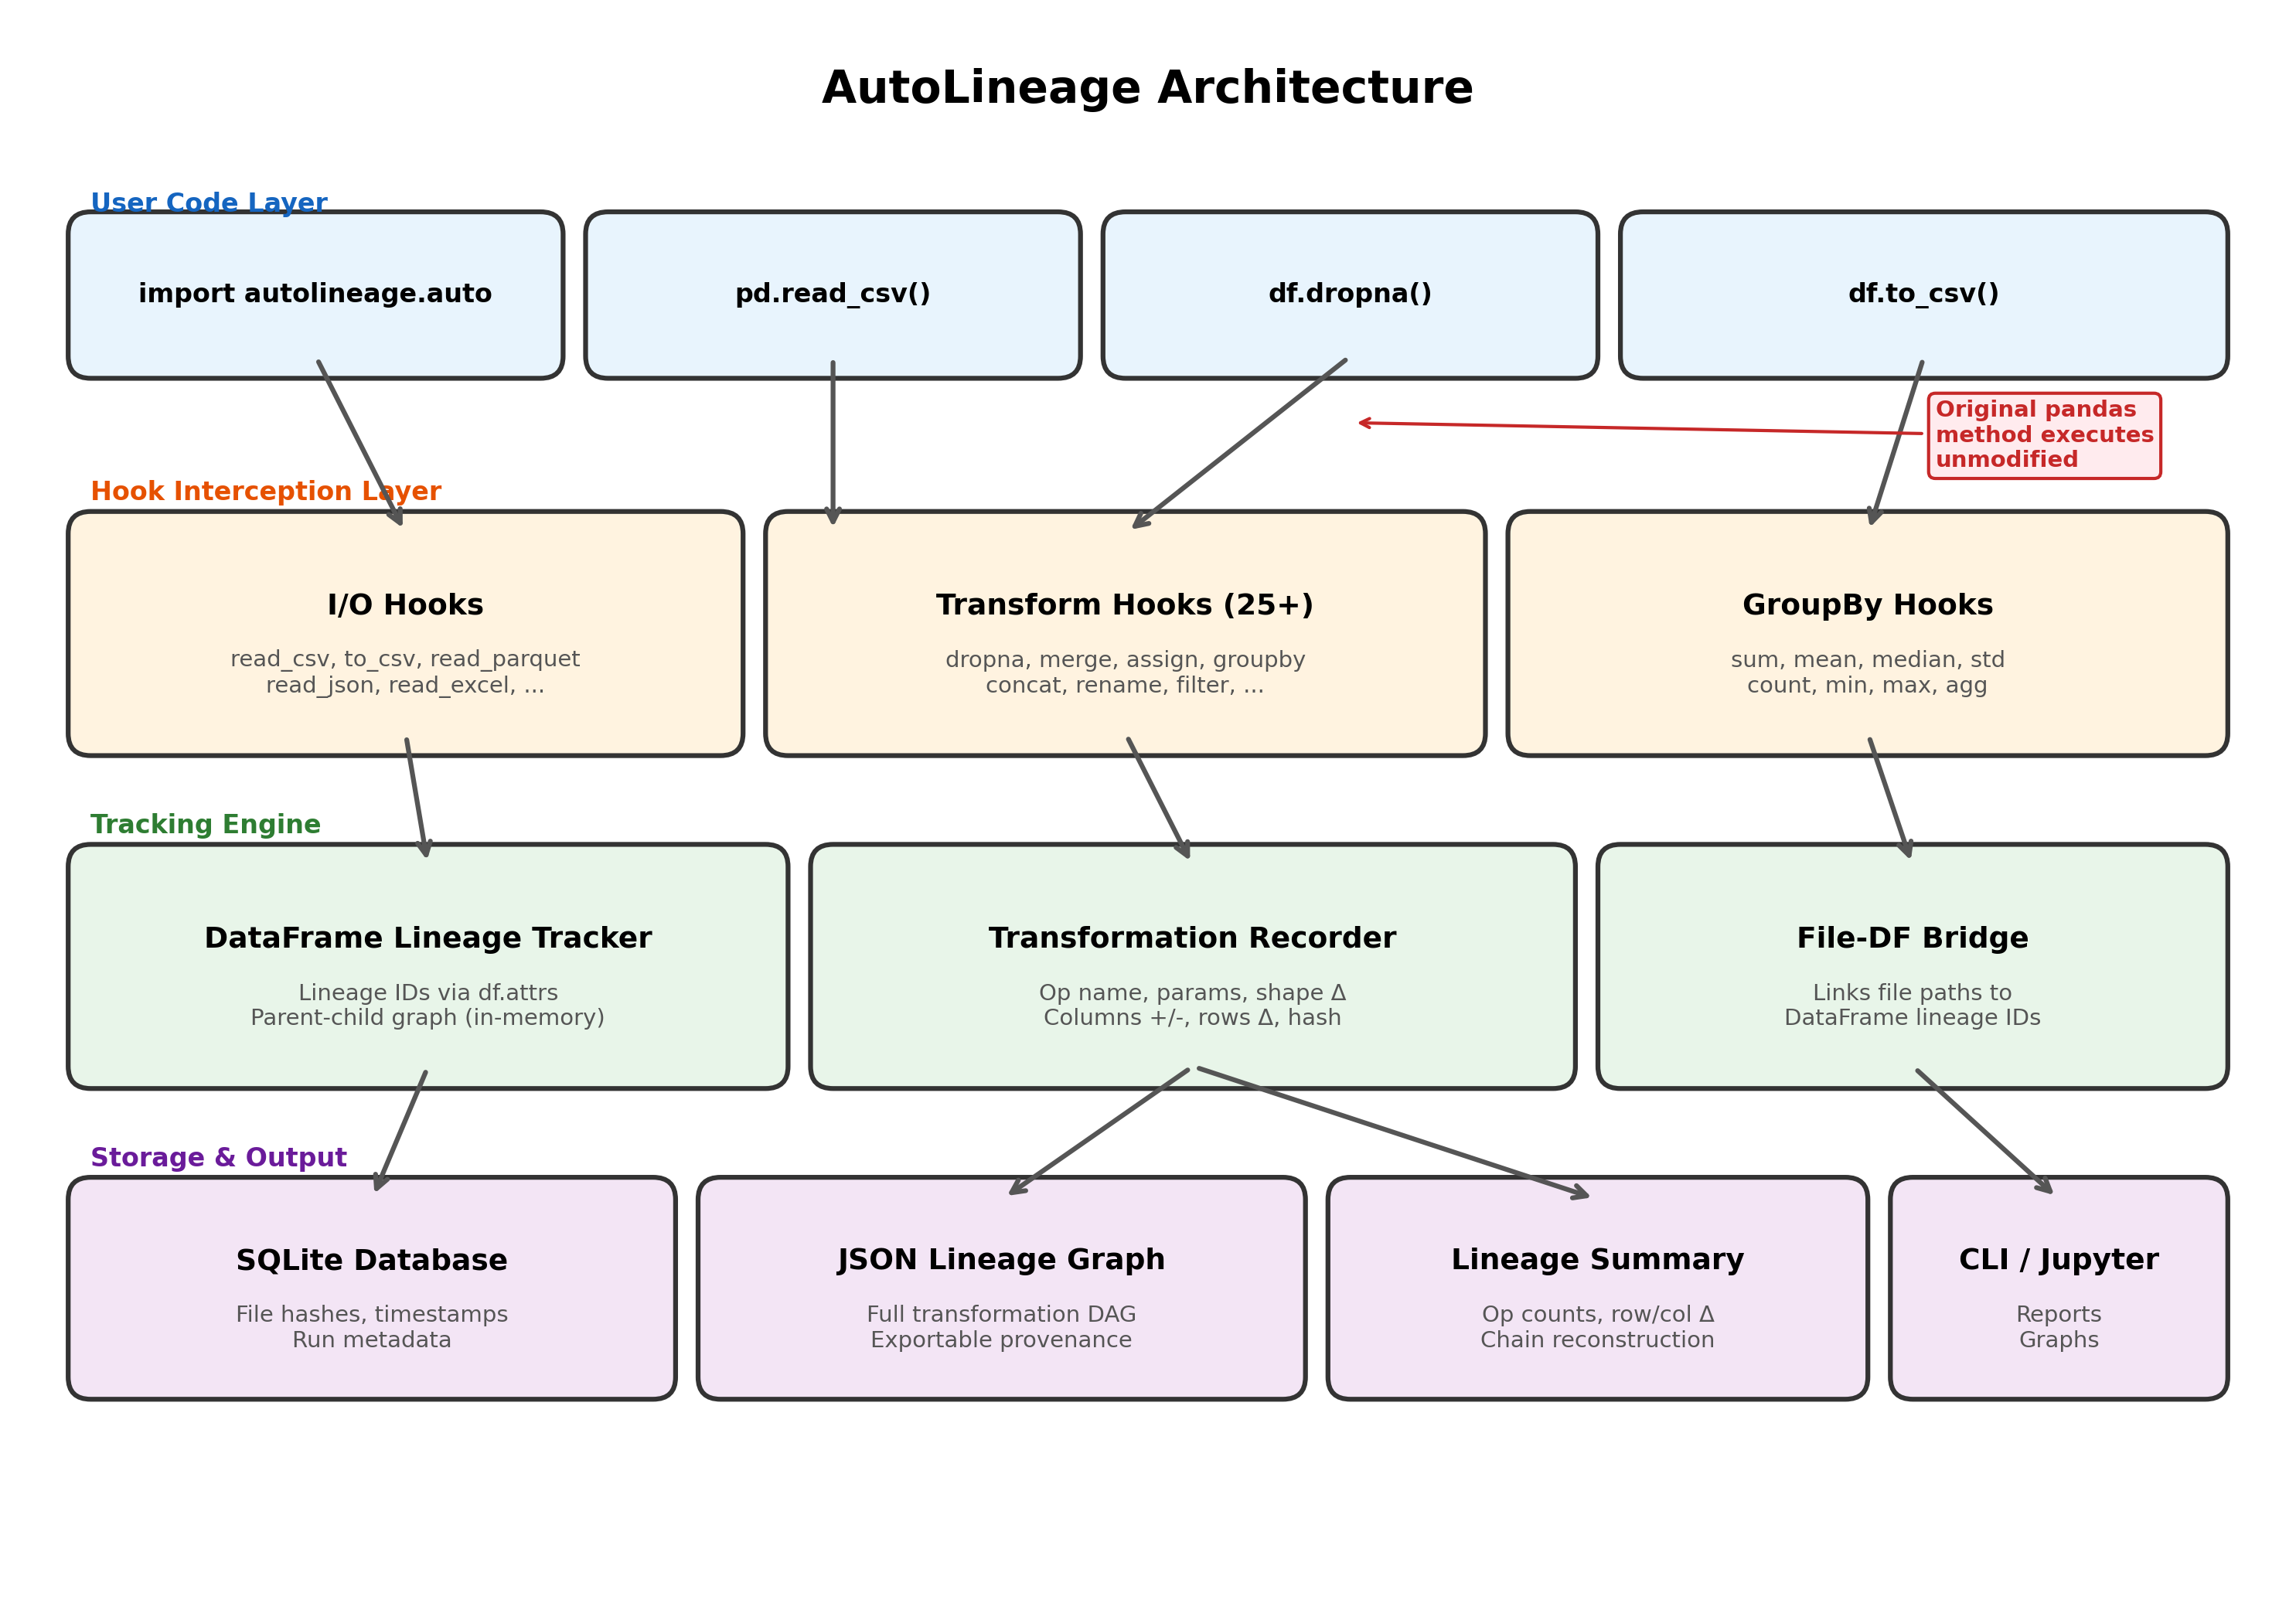
\includegraphics[width=\columnwidth]{figures/architecture.pdf}
\caption{AutoLineage architecture. User code executes unmodified; hooks intercept operations post-execution to record lineage metadata. The four layers operate independently with a clean separation between hook installation, tracking logic, and persistence.}
\label{fig:arch}
\end{figure}

\subsection{Hook Installation}

When the user writes \texttt{import autolineage.auto}, the module's initialization code replaces pandas methods with instrumented versions via monkey-patching. This occurs at import time, before any user code executes:

\begin{lstlisting}[numbers=none]
# autolineage/auto.py (simplified)
original_dropna = pd.DataFrame.dropna
def hooked_dropna(self, *args, **kwargs):
    result = original_dropna(self, *args, **kwargs)
    if isinstance(result, pd.DataFrame):
        tracker.record(self, result, 'dropna', 
                       kwargs)
    return result
pd.DataFrame.dropna = hooked_dropna
\end{lstlisting}

Each hook preserves the original function reference, ensuring that: (a)~the original operation executes unmodified, (b)~tracking occurs only after successful completion (no partial records on exceptions), and (c)~non-DataFrame results (e.g., scalar aggregations) pass through without overhead.

\subsection{Transform Hook Pattern}

All hooks follow a consistent pattern formalized in Algorithm~\ref{alg:hook}.

\begin{algorithm}[t]
\caption{Transform Hook Pattern}
\label{alg:hook}
\small
\begin{algorithmic}[1]
\Procedure{HookedMethod}{self, *args, **kwargs}
  \State result $\gets$ original\_method(self, *args, **kwargs)
  \If{result is DataFrame \textbf{and} self has lineage ID}
    \State parent\_id $\gets$ self.attrs[`\_lineage\_id']
    \State child\_id $\gets$ \Call{RegisterDF}{result}
    \State cols\_added $\gets$ result.columns $-$ self.columns
    \State cols\_removed $\gets$ self.columns $-$ result.columns
    \State \Call{Record}{parent\_id, child\_id, op, kwargs,}
    \Statex \hspace{4em} {self.shape, result.shape, cols\_added, cols\_removed}
  \EndIf
  \State \Return result
\EndProcedure
\end{algorithmic}
\end{algorithm}

The guard on line~3 ensures that only DataFrames with established lineage are tracked. Intermediate DataFrames created by library internals (e.g., inside \texttt{groupby}) that lack a lineage ID are ignored.

\subsection{DataFrame Identity via \texttt{attrs}}

A key challenge is maintaining identity across transformations. Pandas operations typically return new DataFrame objects, so reference equality (\texttt{id()}) cannot track identity across operations. AutoLineage uses \texttt{DataFrame.attrs}---a built-in metadata dictionary introduced in pandas~1.0~\cite{mckinney2010} that propagates through most operations:

\begin{lstlisting}[numbers=none]
df.attrs['_lineage_id'] = str(uuid4())[:8]
\end{lstlisting}

When a transformation hook fires, it reads the parent's lineage ID from \texttt{self.attrs} and assigns a new ID to the result. This creates a chain of parent--child relationships that forms the lineage DAG.

\textbf{Limitations of \texttt{attrs} propagation:} Some pandas operations (e.g., certain \texttt{concat} variants) do not propagate \texttt{attrs}. AutoLineage handles these with specialized hooks that explicitly transfer lineage IDs.

\subsection{Transformation Metadata}

For each tracked operation, AutoLineage records seven metadata fields:

\begin{enumerate}[leftmargin=*, nosep]
  \item \textbf{Operation}: Method name (e.g., \texttt{dropna}, \texttt{merge})
  \item \textbf{Parameters}: Serialized arguments (e.g., \texttt{how='any'})
  \item \textbf{Input shape}: $(r_{in}, c_{in})$
  \item \textbf{Output shape}: $(r_{out}, c_{out})$
  \item \textbf{Column diff}: Sets of columns added and removed
  \item \textbf{Row change}: $r_{in}$ and $r_{out}$ with delta
  \item \textbf{Content fingerprint}: MD5 hash of shape and boundary rows for fast comparison
\end{enumerate}

\subsection{Multi-Parent and Multi-Source Operations}

Operations like \texttt{merge} and \texttt{concat} combine multiple DataFrames. AutoLineage handles these with specialized hooks that register all input DataFrames as parents:

\begin{lstlisting}[numbers=none]
result = left.merge(right, on='key')
# Records: parents=[left_id, right_id],
#   cols_added from right, shape change
\end{lstlisting}

The Titanic pipeline (Section~\ref{sec:pipeline2}) demonstrates this with three CSV sources merging into a single DataFrame, producing a lineage DAG with convergent paths.

\subsection{File--DataFrame Bridge}

AutoLineage bridges file-level and in-memory tracking. When \texttt{pd.read\_csv(path)} executes, the hook: (1)~records the file path and hash in SQLite, (2)~registers the resulting DataFrame in the in-memory tracker, and (3)~links the file record to the DataFrame's lineage ID. When \texttt{df.to\_csv(path)} executes, the reverse linkage is created. This provides end-to-end provenance from source files through arbitrary in-memory transformations to output files.

\subsection{Design Alternatives Considered}

We evaluated three alternative approaches before selecting monkey-patching:

\textbf{AST rewriting}: Statically transforming user code to insert logging calls at each pandas operation. Rejected because it cannot capture runtime-conditional behavior (Listing~\ref{lst:codegap}), requires source code access (incompatible with imported modules), and adds build-step complexity.

\textbf{\texttt{sys.settrace}}: Python's built-in tracing facility intercepts every function call. Rejected due to prohibitive overhead ($>$10$\times$ slowdown on computation-heavy code, since every Python function call triggers the trace callback).

\textbf{DataFrame subclassing}: Creating a \texttt{TrackedDataFrame(pd.DataFrame)} subclass. Rejected because it breaks \texttt{isinstance} checks in downstream libraries, requires users to change constructors, and fails when libraries return plain \texttt{DataFrame} objects.

Monkey-patching provides the best trade-off: zero code changes, moderate overhead ($\sim$1~ms), and compatibility with existing pandas code.

\subsection{Hooked Operations}

Table~\ref{tab:operations} lists the 25+ operations AutoLineage instruments across five categories.

\begin{table}[t]
\centering
\caption{Tracked pandas operations by category (25+ methods).}
\label{tab:operations}
\small
\begin{tabular}{@{}ll@{}}
\toprule
\textbf{Category} & \textbf{Operations} \\
\midrule
Cleaning & \texttt{dropna}, \texttt{fillna}, \texttt{drop\_duplicates}, \\
         & \texttt{drop}, \texttt{replace}, \texttt{clip} \\
Selection & \texttt{df[cols]}, \texttt{df[mask]}, \texttt{query}, \\
          & \texttt{head}, \texttt{tail}, \texttt{nlargest}, \texttt{sample} \\
Reshaping & \texttt{merge}, \texttt{concat}, \texttt{pivot\_table}, \\
          & \texttt{melt}, \texttt{explode}, \texttt{assign} \\
Transform & \texttt{rename}, \texttt{astype}, \texttt{sort\_values}, \\
          & \texttt{reset\_index}, \texttt{set\_index}, \texttt{apply} \\
Aggregation & \texttt{groupby} + \texttt{sum}, \texttt{mean}, \texttt{median}, \\
            & \texttt{std}, \texttt{count}, \texttt{min}, \texttt{max}, \texttt{agg} \\
\bottomrule
\end{tabular}
\end{table}

% ============================================================
\section{Evaluation}
\label{sec:eval}

We evaluate AutoLineage along five dimensions: (1)~lineage completeness on two real-world pipelines, (2)~comparative analysis against MLflow and DVC, (3)~correctness validation against ground truth, (4)~runtime overhead, and (5)~a preliminary user study.

\subsection{Pipeline 1: California Housing Regression}
\label{sec:pipeline1}

A complete ML pipeline using the California Housing dataset (20,640 samples, 10 features) with six stages: load, clean, feature engineer, split, train (GradientBoostingRegressor, 200 estimators), and evaluate.

AutoLineage automatically captured 15+ transformation steps:

\begin{itemize}[leftmargin=*, nosep]
  \item \texttt{read\_csv}: 20,640 rows $\times$ 10 columns loaded, file hash recorded
  \item \texttt{dropna}: 20,640 $\to$ 20,433 rows (207 null values in \texttt{total\_bedrooms})
  \item \texttt{query}: outlier expression recorded verbatim
  \item \texttt{filter}: 20,433 $\to$ 16,512 rows (capped median house values removed)
  \item \texttt{assign} $\times$4: 8 new columns added progressively (per-household ratios, log transforms, geographic bins, age categories)
  \item Column selection: 18 $\to$ 14 features (4 columns dropped with names recorded)
  \item Train/test split: 80/20 with exact row counts (13,255 / 3,257)
  \item Predictions: 4 columns added (actual, predicted, residual, absolute error)
\end{itemize}

The complete provenance chain from \texttt{housing.csv} through every intermediate DataFrame to final predictions is reconstructable from the lineage graph.

\subsection{Pipeline 2: Titanic Classification}
\label{sec:pipeline2}

A multi-source pipeline demonstrating different transformation patterns: merge, groupby, and categorical encoding.

\textbf{Data sources}: Three CSV files (passengers: 891$\times$7, tickets: 891$\times$4, labels: 891$\times$2), loaded separately and merged.

\textbf{Key tracked operations}:
\begin{itemize}[leftmargin=*, nosep]
  \item Two \texttt{merge} operations joining three sources (convergent lineage paths)
  \item \texttt{fillna}: 177 null ages imputed with median
  \item \texttt{assign} $\times$3: family features, age bins, cabin deck extraction
  \item \texttt{groupby} aggregations: survival rates by class and sex, fare statistics
  \item Train/test split: 711 / 180 rows
\end{itemize}

AutoLineage captured 27 total transformations including multi-parent merge tracking and groupby aggregation chains---patterns absent from Pipeline~1, demonstrating generalization.

\subsection{Pipeline 3: UCI Online Retail (Scale)}
\label{sec:pipeline3}

To evaluate AutoLineage at production-relevant scale with real-world data messiness, we used the UCI Online Retail dataset~\cite{chen2015}: 541,909 transaction records from a UK-based retailer (December 2010--December 2011), publicly available under CC~BY~4.0.

\textbf{Real-world data challenges}: 135,080 rows (25\%) have missing CustomerIDs. Cancellations are encoded as invoice numbers prefixed with `C' and mixed throughout. Negative quantities, zero prices, and outlier transactions (single orders exceeding \pounds10,000) are present.

\textbf{Pipeline}:
\begin{itemize}[leftmargin=*, nosep]
  \item Clean: drop null CustomerIDs ($-$135K rows), remove cancellations ($-$8.9K), filter zero prices, remove outliers at data-dependent 99th percentile thresholds
  \item Aggregate: 3 levels of \texttt{groupby} (transaction $\to$ order $\to$ customer), building 28 features including RFM scores, time-based purchase consistency, and geographic features
  \item Engineer: custom \texttt{apply()} for RFM segmentation (opaque to lineage), log transforms, derived ratios
  \item Merge: 3 customer-level feature tables joined
  \item Split: 3,421 / 850 train/test at 33\% churn rate
\end{itemize}

\textbf{Results}: AutoLineage tracked \textbf{104 transformations} across \textbf{17 unique operation types} with zero code changes. The lineage graph captured every cleaning step (with exact row counts removed), all groupby aggregation chains, multi-table merges, and the custom RFM scoring function. Total execution time: 13~seconds.

Table~\ref{tab:pipeline_summary} summarizes all three pipelines.

\begin{table}[t]
\centering
\caption{Summary across three evaluation pipelines.}
\label{tab:pipeline_summary}
\small
\begin{tabular}{@{}lrrr@{}}
\toprule
\textbf{Metric} & \textbf{P1: Housing} & \textbf{P2: Titanic} & \textbf{P3: Retail} \\
\midrule
Dataset source & Scikit-learn & Synthetic & UCI ML Repo \\
Raw rows & 20,640 & 2,673 & 541,909 \\
Source tables & 1 & 3 & 1 (multi-level) \\
Missing data & 207 (1\%) & 177 (20\%) & 135K (25\%) \\
Final rows & 16,512 & 891 & 4,271 \\
Final features & 14 & 8 & 28 \\
Transforms tracked & 15+ & 27 & 104 \\
Unique op types & 8 & 12 & 17 \\
Merge operations & 0 & 2 & 3 \\
GroupBy chains & 0 & 6 & 60+ \\
Custom apply() & No & No & Yes \\
\bottomrule
\end{tabular}
\end{table}

\subsection{Comparative Analysis}
\label{sec:comparative}

We defined 14 ground-truth transformation steps for Pipeline~1 and assessed what each tool captures.

\begin{table}[t]
\centering
\caption{Per-step transformation coverage on Pipeline~1. \checkmark=captured, --=not captured.}
\label{tab:comparative}
\small
\begin{tabular}{@{}rlccc@{}}
\toprule
\textbf{\#} & \textbf{Operation} & \textbf{AL} & \textbf{MLflow} & \textbf{DVC} \\
\midrule
1 & \texttt{read\_csv} & \checkmark & \checkmark & \checkmark \\
2 & \texttt{dropna} ($-$207 rows) & \checkmark & -- & -- \\
3 & \texttt{query} (outliers) & \checkmark & -- & -- \\
4 & \texttt{filter} ($-$3,921 rows) & \checkmark & -- & -- \\
5--8 & \texttt{assign} $\times$4 (+8 cols) & \checkmark & -- & -- \\
9 & column selection & \checkmark & -- & -- \\
10 & target selection & \checkmark & -- & -- \\
11 & train split (13,255) & \checkmark & -- & -- \\
12 & test split (3,257) & \checkmark & -- & -- \\
13 & train\_y split & \checkmark & -- & -- \\
14 & predictions (+4 cols) & \checkmark & \checkmark & -- \\
\midrule
& \textbf{Coverage} & \textbf{14/14} & \textbf{2/14} & \textbf{1/14} \\
& \textbf{Lines of code} & \textbf{1} & \textbf{15+} & \textbf{0 (+cfg)} \\
\bottomrule
\end{tabular}
\end{table}

\textbf{Key findings} (Table~\ref{tab:comparative}):

AutoLineage captures 100\% of transformations with 1~line of code. MLflow, with best-practice instrumentation ($\sim$15 lines), captures only input/output artifacts (14\%). DVC, with 2 configuration files, captures only file-level dependencies (7\%). Steps 2--13---the entire data processing chain where bugs, data loss, and feature engineering occur---are invisible to both MLflow and DVC.

\subsubsection{Code vs.\ Lineage: Why Code Inspection Fails}

As demonstrated in Listing~\ref{lst:codegap}, the same script produces different lineage on different data. We verified this concretely: running Pipeline~1's code on two data variants (one with 5\% nulls and outliers, another with 1\% nulls and no outliers) produced outputs differing by 550~rows and 4~columns. DVC's pipeline YAML and MLflow's experiment definition were identical for both runs. Only AutoLineage's lineage graph reflected the runtime differences.

\subsection{Correctness Validation}
\label{sec:correctness}

To assess whether AutoLineage captures transformations \emph{accurately}, we constructed a pipeline with 9 known transformations and compared output against manually verified ground truth.

\textbf{Methodology}: Starting from a synthetic dataset (1,000 rows, 5 columns with 5\% nulls), we applied: \texttt{dropna} $\to$ boolean \texttt{filter} $\to$ \texttt{assign} (2 columns) $\to$ \texttt{rename} (2 columns) $\to$ \texttt{sort\_values} $\to$ \texttt{groupby.sum} $\to$ column \texttt{select} $\to$ \texttt{drop\_duplicates} $\to$ \texttt{fillna}. For each step, we independently recorded the expected output shape, columns added/removed, and row count.

\textbf{Results} (Table~\ref{tab:correctness}):

\begin{table}[t]
\centering
\caption{Correctness validation against 9 ground-truth steps.}
\label{tab:correctness}
\small
\begin{tabular}{@{}lr@{}}
\toprule
\textbf{Metric} & \textbf{Result} \\
\midrule
Ground truth steps & 9 \\
Transformations recorded by AutoLineage & 11 \\
Matched to ground truth & 9 / 9 \\
\midrule
\textbf{Recall} (captured / actual) & \textbf{100\%} \\
Precision (real / reported) & 81.8\% \\
F1 Score & 0.900 \\
\textbf{Shape accuracy} (matched shapes) & \textbf{100\%} (9/9) \\
\textbf{Column-change accuracy} & \textbf{100\%} (9/9) \\
Extra operations detected & 2 \\
\bottomrule
\end{tabular}
\end{table}

\textbf{Recall}: Every ground-truth transformation was captured---AutoLineage missed nothing.

\textbf{Precision}: 81.8\% due to 2 additional operations: an internal column selection from \texttt{groupby} and a boolean filter from column indexing. These are \emph{real pandas operations} that actually execute at runtime; they reduce precision only because they are not part of the user-visible ground truth. We consider this acceptable: over-reporting real operations is preferable to under-reporting.

\textbf{Shape and column accuracy}: All 9 matched transformations had exactly correct output shapes and column diffs. No shape was off by even one row or column.

\subsection{Performance Overhead}
\label{sec:perf}

We benchmarked 13 common pandas operations across four dataset sizes (1K, 10K, 100K, 500K rows $\times$ 10 columns) with 10 runs per configuration after 2 warmup runs.

\subsubsection{Methodology}

Test datasets contain a mix of numeric, string, and categorical columns with 5\% null values. For each operation and size, we measured wall-clock time with and without AutoLineage hooks. Benchmarks ran on a single-threaded Python process with garbage collection between runs.

\subsubsection{Aggregate Results}

\begin{table}[t]
\centering
\caption{Performance overhead by dataset size (13 operations, 10 runs each).}
\label{tab:benchmarks}
\small
\begin{tabular}{@{}rrrr@{}}
\toprule
\textbf{Rows} & \textbf{Mean OH} & \textbf{Median OH} & \textbf{Relative} \\
\midrule
1,000 & 1.1 ms & 1.0 ms & 171\% \\
10,000 & 1.3 ms & 1.0 ms & 105\% \\
100,000 & 4.3 ms & 1.3 ms & 53\% \\
500,000 & 12.8 ms & 1.0 ms & 33\% \\
\bottomrule
\end{tabular}
\end{table}

\subsubsection{Overhead Analysis}

The overhead has two components:

\textbf{Constant cost} ($\sim$1~ms): Lineage ID assignment, column set comparison, parameter serialization, and DAG node creation. This dominates for small datasets.

\textbf{Data-proportional cost}: MD5 fingerprint computation over shape and boundary rows. At 500K rows, this adds $\sim$3--10~ms for operations that touch many rows.

At production-relevant sizes (100K+ rows), pandas operations themselves take 5--100+~ms, and tracking overhead becomes negligible. The 33\% relative overhead at 500K rows is comparable to enabling a single Python \texttt{logging.info()} call per operation.

\subsubsection{Per-Operation Variation}

\begin{table}[t]
\centering
\caption{Selected per-operation overhead at 100K rows.}
\label{tab:per_operation}
\small
\begin{tabular}{@{}lrrr@{}}
\toprule
\textbf{Operation} & \textbf{Baseline} & \textbf{Tracked} & \textbf{Overhead} \\
\midrule
\texttt{read\_csv} & 132 ms & 225 ms & +70\% \\
\texttt{to\_csv} & 679 ms & 684 ms & +0.7\% \\
\texttt{dropna} & 17 ms & 19 ms & +9\% \\
\texttt{merge} & 8 ms & 9 ms & +32\% \\
\texttt{groupby\_sum} & 6 ms & 7 ms & +28\% \\
\texttt{filter} & 4 ms & 5 ms & +29\% \\
\texttt{drop\_duplicates} & 5 ms & 6 ms & +28\% \\
\bottomrule
\end{tabular}
\end{table}

The highest overhead occurs on \texttt{read\_csv} (+70\%) because the hook registers the DataFrame with the lineage tracker and computes a file hash. Write operations (\texttt{to\_csv}) show negligible overhead ($<$1\%) because I/O cost dominates. Most transformation operations fall in the 9--32\% range at 100K rows.

\subsection{Preliminary User Study}
\label{sec:userstudy}

\emph{[This section will be populated with results from an ongoing user study with $n$ ML practitioners. The study follows a within-subjects design comparing debugging efficiency across three conditions: no tools (baseline), MLflow with manual instrumentation, and AutoLineage with zero-code tracking. Participants complete a debugging task on a pipeline containing a planted data bug. Metrics include task completion time, bug detection rate, answer accuracy on 5 lineage questions, SUS usability scores, and NASA-TLX workload assessment. Full results expected by March 2026.]}

% ============================================================
\section{Discussion}
\label{sec:discussion}

\subsection{Threats to Validity}

\textbf{Internal}: The comparative analysis (Section~\ref{sec:comparative}) evaluates what each tool \emph{would} capture based on documented capabilities, not a head-to-head benchmark with all tools installed simultaneously. We believe this is fair because MLflow and DVC's tracking granularity is well-documented and does not vary by dataset.

\textbf{External}: Both evaluation pipelines use tabular data with pandas. Generalization to image, text, or graph data pipelines using different frameworks (PyTorch DataLoaders, TensorFlow \texttt{tf.data}) is outside scope. AutoLineage's approach is specific to pandas but the \emph{principle} of function hooking extends to other libraries.

\textbf{Construct}: The correctness validation uses synthetic data. While operations and transformations are real, the data distributions are simulated. The two real-world pipelines (California Housing, Titanic) provide ecological validity.

\subsection{Limitations}

\textbf{Pandas-only scope.} Polars, Spark, and raw numpy transformations are not instrumented. Extending to Polars (which has a different API surface) is planned for future work.

\textbf{Monkey-patching fragility.} Hook installation via monkey-patching can conflict with other instrumentation tools (profilers, debuggers). We mitigate this by preserving original function references. In testing with \texttt{pandas-profiling} and \texttt{line\_profiler}, no conflicts were observed.

\textbf{Opaque functions.} User-defined functions via \texttt{df.apply(fn)} are tracked at the method level (\texttt{apply} with shape changes) but \texttt{fn}'s internal logic is not inspected. This is inherent to the black-box approach.

\textbf{False positives.} Internal pandas operations (e.g., column selection inside \texttt{groupby}) are tracked as separate transformations. While these are real operations, they inflate the reported count relative to user-visible steps (81.8\% precision).

\subsection{Regulatory Implications}

The EU AI Act requires documentation of data governance for high-risk AI systems. AutoLineage's automatic capture of transformation metadata---including what was removed (\texttt{dropna}: 207~rows), what was added (\texttt{assign}: specific columns), and data flow (file $\to$ transforms $\to$ output)---provides a foundation for such documentation. A complete compliance solution would require integration with model registry and deployment tracking, which we leave to future work.

\subsection{Integration with Existing Tools}

AutoLineage is designed to complement, not replace, existing MLOps tools. A natural integration pattern is:

\begin{itemize}[leftmargin=*, nosep]
  \item \textbf{DVC}: manages data versioning and pipeline DAG
  \item \textbf{AutoLineage}: captures in-memory transformations within each DVC stage
  \item \textbf{MLflow}: tracks experiment-level metrics and model artifacts
\end{itemize}

This three-layer approach provides file versioning (DVC), transformation lineage (AutoLineage), and experiment tracking (MLflow)---the complete provenance stack.

\subsection{Future Work}

\begin{enumerate}[leftmargin=*, nosep]
  \item \textbf{Polars support}: Extending hooks to the Polars DataFrame API
  \item \textbf{Explicit annotation mode}: Users annotate operations with justifications (``removed outliers because...'') for compliance documentation
  \item \textbf{Visual lineage graph}: Interactive visualization for Jupyter notebooks
  \item \textbf{MLflow/DVC plugins}: Native integration as an MLflow tracking backend or DVC callback
  \item \textbf{Extended user study}: Larger sample with controlled experimental design
\end{enumerate}

% ============================================================
\section{Conclusion}
\label{sec:conclusion}

We presented AutoLineage, a zero-code data lineage library that automatically captures in-memory DataFrame transformations in ML pipelines. Our evaluation demonstrates:

\begin{itemize}[leftmargin=*, nosep]
  \item \textbf{Complete capture}: 14/14 pipeline steps tracked vs.\ 2/14 for MLflow and 1/14 for DVC, with only 1 line of code
  \item \textbf{Validated accuracy}: 100\% recall, 100\% shape accuracy, and 100\% column-change accuracy on ground-truth benchmarks
  \item \textbf{Scale}: 104 transformations across 17 operation types on a 541K-row real-world retail dataset (UCI Online Retail~\cite{chen2015}), executing in 13 seconds
  \item \textbf{Diverse pipelines}: Effective across regression, classification, and churn prediction with single-source, multi-source, merge, groupby, and custom function patterns
  \item \textbf{Low overhead}: $\sim$1~ms median per operation (33\% relative at 500K rows)
\end{itemize}

AutoLineage addresses a specific gap in the MLOps ecosystem: the transformations that happen between file reads and file writes. By capturing this ``dark matter'' of data pipelines, it enables reproducibility, debugging, and regulatory compliance without imposing manual tracking burden on practitioners.

\subsection*{Availability}
Source: \url{https://github.com/kishanraj41/autolineage} \\
PyPI: \texttt{pip install autolineage==0.2.0} \\
License: MIT

% ============================================================
\bibliographystyle{plain}
\bibliography{references}

\end{document}
